\section{Méthodes d'organisation \& planification}
Au vu de l'envergure de notre projet, nous sommes obligés de prévoir une planification la plus détaillée possible, qui tienne compte de toutes les tâches qui compoeront la réalisation de notre application, accompagnées de la charge de travail que nous estimons devoir fournir pour les réaliser. Nous devons aussi convenir d'une organisatio rigoureuseLes différents livrables qui nous sont demandés feront office de jalons tout au long de notre projet. 

\subsection{Planification prévisionnelle}
Voici le planing, tel que nous l'avions estimé lors de notre 1\up{er} rapport : \newline
\begin{tabular}{|l|l|}
\hline
  Date &
  Production \\
\hline
  9 janvier &
  Version PC \textnumero2 \\
\hline
  6 février &
  Rapport de conception logicielle VP \\
\hline
  9 février &
  Version PC \textnumero3 \\
\hline
  12 février &
  Rapport de conception logicielle VF \\
\hline
  9 mars &
  Version PC \textnumero4 \\
\hline
  25 mars &
  Page HTML VP \\
\hline
  2 avril &
  Page HTML VF \\
\hline
  9 avril &
  Version PC \textnumero5 \\
\hline
  16 mai &
  Documentation en Ligne VP \\
\hline
  21 mai &
  Rapport Final/Annexes + Bilan Planification \\
\hline
  26 mai &
  Rapport Final/Annexes + Bilan Planification \\
\hline
  28 mai &
  Documentation en Ligne VF \\
\hline
\end{tabular}

\subsection{Méthode agile \& cycle en V}
Au cours du projet, nous allons devoir produire plusieurs livrables, 6 rapports, documentation en ligne, page HTML de présentation ainsi que des versions préliminaires de notre application. Les dates auxquelles ces livrables sont dus sont fixées à l'avance et font office de jalons communs à tous les projets, nous incitant à adopter un développement de type cycle en V (cf. \textsc{figure~\ref{cycle_v}}). En effet les différents livrables correspondent aux différentes étapes du cycle. 
\begin{figure}[h]
  \centering
  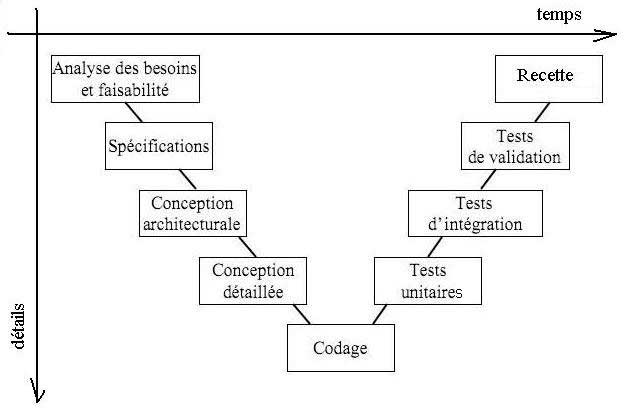
\includegraphics[width=\linewidth]{3-Planification/img-utilisateur/cycle_v}
  \caption{Schéma typique d'un cycle en V}
  \label{cycle_v}
\end{figure}

Pourtant, nous conformer uniquement à ce type de cycle nous paraissait limitatif. Notre groupe est composé de 7 personnes, ce qui représente plus de ressources que nécessaires pour une partie des livrables et permet de répartir une partie de nos effectifs sur la conception pendant que l'autre réalise les livrables. L'emploi d'une méthode agile nous permet de nous approcher au plus près possible des attentes de nos clients du centre de Kerpape en leur présentant régulièrement l'avancement de notre application et en discutant avec eux d'éventuels changements à apporter.\newline

Nous ne nous cantonnerons pas à une seule méthode d'organisation, mais profiterons du meilleur que chacune d'elles peut apporter pour respecter les différents jalons fixés tout en offrant le meilleur résultat possible au centre de Kerpape. 

\subsection{Organisation}

Notre groupe se composera, à partir du 2\up{ème} semestre, de 5 étudiants. Nous estimons que, compte tenu du temps requis par les cours et les autres projets, nous pouvons fournir environ 7h de travail/personne/semaine, soit au total 35h/semaine. \newline

Nous n'avons pas de chef de projet attitré tout au long de l'année. La politique que nous avons employée jusque là et que nous conserverons est qu'à chaque phase du projet, matérialisée par un rapport ou bien la soutenance finale, l'un des membres de l'équipe s'occupera de la fonction de chef de projet. Il s'agira avant tout de gérer les livrables et de piloter l'équipe, car les décisions importantes concernant l'architecture logicielle et le développement du projet seront prises en groupe. Cela permet à chacun d'entre nous d'assurer tour à tour la responsabilité de chef d'équipe et en même temps que tous soient responsables de l'aspect final que prendra le projet Avalon. 